\سؤال{}

\textbf{تصور کنید که پس از اتمام تحصیل تصمیم به راه‌اندازی شرکتی نرم‌افزاری با دوستانتان گرفته‌اید. ساختار این شرکت از لحاظ نیروی انسانی به چه شکلی است؟ چه نیروهایی دارد؟ می‌توانید برای پاسخ‌گویی بهتر حوزه فعالیت شرکت را به دل‌خواه پیش‌نهاد دهید. مثلا بگویید شرکت بناست در حوزه تولید نرم‌افزارهای مالی فعالیت کند لذا این نیروها را خواهد خواست. }
\newline

\begin{itemize}
	\item الف)
	ساختار تیم نیروی انسانی به یکی از ۴ شکل زیر است: 
	\begin{enumerate}
		\item الگوی بسته \footnote{\lr{closed paradigm}}
		در این الگو، تیم به‌طور شکل سنتی و سلسله‌مراتبی دارد. این‌گونه تیم‌ها در هنگام تولید و ایجاد نرم‌افزار که شبیه کارهای گذشته باشد، به خوبی کار می‌کند. اما احتمال نوآورانه بودن آن در این الگوی بسته بسیار پایین است. 
		\item الگوی تصادفی \footnote{\lr{random paradigm}} د
		در این الگو یک تیم به نوآوری و  ابتکار فردی اعضای تیم وابستگی زیادی دارد. این الگو وقتی مزیت دارد که دست‌یابی به یک نوآوری یا موقعیت تکنولوژیکی مورد نیاز است. اما این متدولوژی هنگامی که عمل‌کرد منظم مطرح و ضروری می‌شود، عملکرد خوبی ندارد.
		\item الگوی باز\footnote{\lr{open paradigm}}
		در این الگو، سعی در ساختاربندی تیم به شکلی داریم که به برخی از کنترل‌های مرتبط با الگوی بسته دست یابد؛ هم‌چنین نوآوری‌های زیادی هنگام استفاده از الگوی تصادفی اتفاق می‌افتند. کارها با همکاری مشترک، ارتباطات سنگین و تصمیم‌گیری مبتنی بر تصمیم مشترک در مورد علائم تجاری تیم‌های با الگوی باز انجام می‌شود. ساختار تیم الگوی باز برای بسیاری از مسائل پیچیده مناسب است اما ممکن استبه اندازه سایر تیم‌ها کارآمد نباشد. 
		\item الگوی هماهنگ
		\footnote{\lr{synchronous paradigm}} 
		 این الگو متکی‌به تقسیم طبیعی یک مسئله است و اعضای تیم را برای داشتن ارتباط فعال با یک‌دیگر کمک می‌کند.
	\end{enumerate}
	\item در این سوال فرض می‌کنیم از متدولوژی چابک برای تشکیل روند تیم استفاده کنیم. استفاده از این متدولوژی باعث می‌شود تیم ساختار سلسله مراتبی داشته باشد و نقش‌ها در آن به شکل زیر است:
	\begin{figure}[!h]
		\begin{center}
			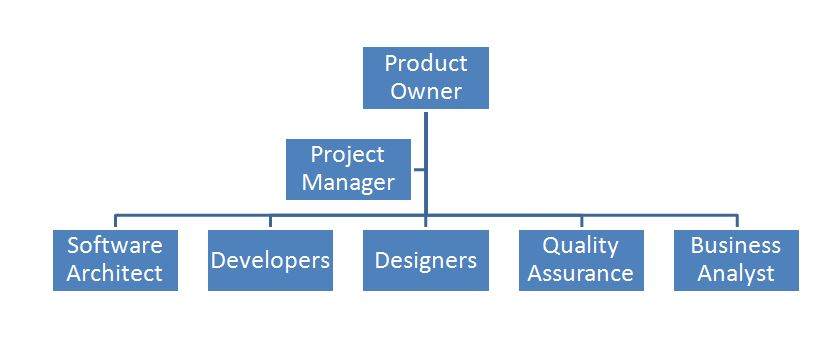
\includegraphics[width=\linewidth]{./5.jpg}
			\caption{ساختار تیم ایجاد و توسعه}
		\end{center}
	\end{figure}
	\item 
	در این سوال فرض شده است که می‌خواهیم یک سامانه حمل‌ونقل بار بین شهری ایجاد کنیم. به همین منظور در متدولوژی \lr{Agile}، نقش‌های مختلفی در تیم وجود دارد. برای مثال صاحب محصول\footnote{\lr{Product Owner }} همان مشتری است که با ما برای انجام پروژه در ارتباط است، محدودیت‌های مالی و زمانی را تعیین می‌کند و مطابق پروپوزال او، باید برنامه‌های تعیین نیازمندی‌های پروژه استخراج شود و سپس برنامه‌ی مدونی به او داده شود.
	
\end{itemize}